% This file was created by tikzplotlib v0.9.4.
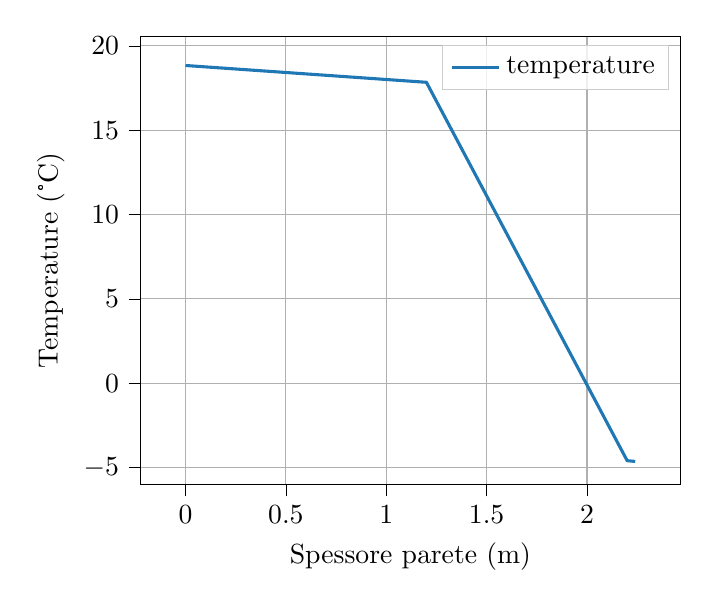
\begin{tikzpicture}

\definecolor{color0}{rgb}{0.12156862745098,0.466666666666667,0.705882352941177}

\begin{axis}[
legend cell align={left},
legend style={fill opacity=0.8, draw opacity=1, text opacity=1, draw=white!80!black},
tick align=outside,
tick pos=left,
x grid style={white!69.0196078431373!black},
xlabel={Spessore parete (m)},
xmajorgrids,
%xmin=-0.0185, xmax=0.3885,
xtick style={color=black},
y grid style={white!69.0196078431373!black},
ylabel={Temperature (°C)},
ymajorgrids,
ymin=-6.01137676302392, ymax=20.5685707562642,
ytick style={color=black}
]
\addplot [line width=1.12pt, color0]
coordinates {%
( 0.0 , 18.833499501495513 )
( 1.2000000000000002 , 17.836490528414757 )
( 2.2 , -4.596211365902292 )
( 2.24 , -4.641076769690926 )
};
\addlegendentry{temperature}
\end{axis}

\end{tikzpicture}

\begin{figure}[htb]
    \centering
    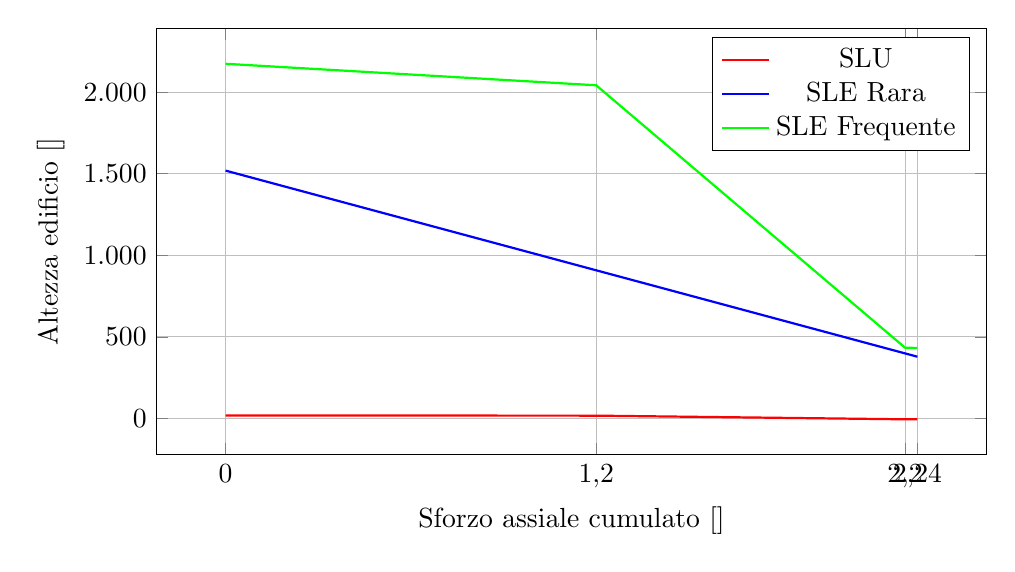
\begin{tikzpicture}
        \begin{axis}[
            /pgf/number format/.cd,
            use comma,      %virgola nei decimali
            %1000 sep={\,},  %uno spazio nelle migliaia
            width=\textwidth,
            height=7cm,
            grid=major,
            xlabel=Sforzo assiale cumulato \si{[\kilo\newton]},
            ylabel=Altezza edificio \si{[\meter]},
            %ytick = {9.7,6.6,3.5,0,-2.75},
            xtick = {0.   , 1.2  , 2.2  , 2.24}
            %title=Titolo se serve
        ]
        \addplot[thick,color=red] coordinates {
            ( 0.0 , 18.833499501495513 )
            ( 1.2000000000000002 , 17.836490528414757 )
            ( 2.2 , -4.596211365902292 )
            ( 2.24 , -4.641076769690926 )
        };
        \addplot[thick,color=blue] coordinates {
            ( 0.0 , 1519.06408007576 )
            ( 1.2000000000000002 , 908.24992313153 )
            ( 2.2 , 399.23812567800496 )
            ( 2.24 , 378.877653779864 )
        };
        \addplot[thick,color=green] coordinates {
            ( 0.0 , 2173.505604685474 )
            ( 1.2000000000000002 , 2041.7740689579205 )
            ( 2.2 , 434.0608608536207 )
            ( 2.24 , 432.58930579824687 )
        };
        \legend{SLU,SLE Rara,SLE Frequente,SLE Quasi Permanente}
        \end{axis}
    \end{tikzpicture}
    \caption{Andamento dello sforzo assiale agente sul pilastro P27 in funzione dell'altezza}
    \label{fig:AndamentoP27}
    \end{figure}